\documentclass[a4paper,11pt,exos]{nsi} % COMPILE WITH DRAFT
\usepackage{pifont}
\usepackage{fontawesome5}
\usepackage{hyperref}

\pagestyle{empty}

\begin{document}
\classe{\premiere spé}
\titre{Préparation à l'évaluation-bilan 5}
\maketitle

\exo{ Concentration d'un antibiotique}
On étudie la concentration dans le sang en fonction du temps d'un antibiotique injecté en une seule prise à un patient. On modélise cette concentration par la fonction $g$ définie sur l'intervalle $\fif{0}{10}$ par : $\quad g(t)=\dfrac{4t}{t^2+1}$.\\
$g(t)$ représente la concentration en mg.L$^{-1}$ de l'antibiotique lorsquer $t$ heures se sont écoulées.\\[.5em]
Répondre aux questions suivantes de façon algébrique. Il est possible de vérifier la cohérence des résultats à l'aide d'un graphique à la calculatrice.
\begin{enumerate}
    \item On cherche à déterminer sur quel intervalle de temps la concentration sera supérieure ou égale à 1,6 mg.L$^{-1}$.
        \begin{enumalph}
            \item Montrer que résoudre l'inéquation $\quad g(t)\geqslant 1,6 \quad$ revient à résoudre l'inéquation\\ $\quad -1,6t^2+4t-1,6\geqslant 0$.
            \item Résoudre l'inéquation $\quad -1,6t^2+4t-1,6\geqslant 0\quad$ et conclure : sur quel intervalle de temps la concentration sera-t-elle supérieure ou égale à 1,6 mg.L$^{-1}$ ?
        \end{enumalph}

    \item On cherche à determiner si concentration peut être strictement supérieure à 2 mg.L$^{-1}$.
    \begin{enumalph}
        \item Montrer que résoudre l'inéquation $\quad g(t)>2 \quad$ revient à résoudre l'inéquation\\ $\quad -2t^2+4t-2> 0$.
        \item Résoudre l'inéquation $\quad -2t^2+4t-2> 0\quad$ et conclure : la concentration peut-elle être strictement supérieure à 2 mg.L$^{-1}$ ?
    \end{enumalph}
\end{enumerate}




\newpage

\dleft{10cm}{
    \exo{}
    La courbe ci-contre représente dans un repère du plan une fonction $f$ définie et dérivable sur l'ensemble des nombres réels.

    Les points G$(-2~;~5)$ et H $(0~;~1)$ appartiennent à  la courbe représentative de la fonction $f$ et les tangentes à  la courbe aux points G et H sont horizontales.\\

    Le but de l'exercice est de déterminer l'expression algébrique de la fonction $f$.
}{\includegraphics[width=6.4cm]{courbe.jpg}}





\begin{enumerate}
\item Déterminer $f(0),\, f(-2), f'(0)$ et $f'( -2)$.
\item  On admet que pour tout réel $x$\,, $f(x)$ peut s'écrire sous la forme :
$$f(x) = ax^3 +bx^2 +cx +d,$$

où \: $a,\, b,\, c$ \: et\: $d$\: désignent des nombres réels .


	\begin{enumalph}
		\item Donner une expression de $f'(x)$ à l'aide de $a,b,c$ et $d$.
    \item Traduire $f(0)=1$ par une égalité sur les coefficients $a,b,c$ et $d$ et en déduire la valeur de $d$.
    Traduire $f'(0)=0$ par une égalité et en déduire la valeur de $c$.
    Conclure : \\
    Pour tout $x\in \R, f(x)= ax^3+bx^2+ .........................\quad$ et $\quad f'(x)=$\dotfill
    \item Traduire $f(-2)=5$ par une égalité sur les coefficients $a$ et $b$.
    Traduire $f'(-2)=0$ par une égalité sur les coefficients $a$ et $b$.
    \item Résoudre le système $\quad (S):\left\{
        \begin{array}{l}
            \ -8a+4b=4 \\
            \ 12a-4b=0 \\
        \end{array} \right.$\\[.5em]
    Conclure en donnant l'expression de $f(x)$ pour tout $x\in\R$.
	\end{enumalph}
\end{enumerate}

\newpage
\titre{Corrigé de la prép° à l'éval-bilan 5}
\maketitle

\setcounter{section}{0}

\exo{ Concentration d'un antibiotique}
\begin{enumerate}
    \item 
        \begin{enumalph}
            \item Soit $t\in\fif{0}{10}$.
            \begin{tabbing}
                $g(t)\geqslant 1,6$ \= $\iff \dfrac{4t}{t^2+1}\geqslant 1,6$\\[.5em]
                \> $\iff 4t\geqslant 1,6(t^2+1)\quad$ car $t^2+1>0$.\\[.5em]
                \> $\iff 4t\geqslant 1,6t^2+1,6$\\[.5em]
                \> $\iff 0\geqslant 1,6t^2-4t+1,6$
            \end{tabbing}
            \item On résout l'inéquation $\ 1,6t^2-4t+1,6\leqslant 0$.\\
            Calcul du discriminant :\\
            $\Delta = (-4)^2-4\times 1,6\times 1,6$\\
            $\phantom{\Delta} = 16-10,24$\\
            $\phantom{\Delta} = 5,76$\\

            Calcul des racines :
            \begin{multicols}{2}
                $t_1 = \dfrac{4-\sqrt{5,76}}{2\times 1,6}$\\[.5em]
                $\phantom{t_1} = \dfrac{4-2,4}{3,2}$\\[.5em]
                $\phantom{t_1} = 0,5$\\
                $t_2 = \dfrac{4+\sqrt{5,76}}{2\times 1,6}$\\[.5em]
                $\phantom{t_2} = \dfrac{4+2,4}{3,2}$\\[.5em]
                $\phantom{t_2} = 2$\\
            \end{multicols}
            
            On a donc :
            \begin{center}
                \begin{tikzpicture}
                \tkzTabInit[color,lgt=5,espcl=2]
                {$t$ /1, Signe de $1{,}6t^2-4t+1{,}6$ /1}
                {0,0{,}5, 2,10}
                \tkzTabLine{,+,z,-,z,+,}
                \end{tikzpicture}
                \end{center}
           
            L'ensemble des solutions de l'inéquation $\ 1,6t^2-4t+1,6\leqslant 0$ est $\fif{0,5}{2}$.\\[.5em]
            La concentration sera donc supérieure ou égale à 1,6 mg.L$^{-1}$  entre 30 min et 2 h après la prise de l'antibiotique.
        \end{enumalph}
        
        \item \begin{enumalph}
            \item Soit $t\in\fif{0}{10}$.
            \begin{tabbing}
                $g(t)>2$ \= $\iff \dfrac{4t}{t^2+1}>2$\\[.5em]
                \> $\iff 4t>2(t^2+1)\quad$ car $t^2+1>0$.\\[.5em]
                \> $\iff 4t>2t^2+2$\\[.5em]
                \> $\iff 0>2t^2-4t+2$.
            \end{tabbing}
            \item On résout l'inéquation $\ 2t^2-4t+2<0$.\\
            Calcul du discriminant :\\
            $\Delta = (-4)^2-4\times 2\times 2$\\
            $\phantom{\Delta} = 16-16$\\
            $\phantom{\Delta} = 0$\\

            Calcul de la racine :\\
            $t_0 = \dfrac{4}{2\times 2}$\\[.5em]
            $\phantom{t_0} = 1$\\

            On a donc :
            \begin{center}
                \begin{tikzpicture}
                \tkzTabInit[color,lgt=5,espcl=2]
                {$t$ /1, Signe de $2t^2-4t+2$ /1}
                {0,1,10}
                \tkzTabLine{,+,z,+,}
                \end{tikzpicture}
                \end{center}
            
            L'inéquation $\ 2t^2-4t+2<0$ n'a pas de solution.\\[.5em]
            La concentration ne peut donc pas être strictement supérieure à 2 mg.L$^{-1}$.
        \end{enumalph}
\end{enumerate}

\exo{}
\begin{enumerate}
    \item Par lecture graphique, on a :
    \begin{multicols}{4}
        \begin{enumerate}[label=\textbullet]
            \item $f(0)=1$ ;
            \item $f(-2)=5$ ;
            \item $f'(0)=0$ ;
            \item $f'(-2)=0$.
        \end{enumerate}
    \end{multicols}
    
    \item \begin{enumalph}
        \item Soit $x\in\R$.
        \begin{tabbing}
            $f'(x)$ \= $= ax^3+bx^2+cx+d$\\
            \> $=a\times 3x^2+b\times 2x+c\times 1+0$\\
            \> $= 3ax^2+2bx+c$.
        \end{tabbing}

        \item \begin{tabbing}
            $f(0)=1\quad$ \= $\iff \quad a\times 0^3+b\times 0^2+c\times 0+d=1$\\
            \> $\iff\quad d=1$\\[1em]
            $f'(0)=0$ \= $\iff \quad 3a\times 0^2+2b\times 0+c=0$\\
            \> $\iff\quad c=0$
        \end{tabbing}

        On a donc $\quad f(x)=ax^3+bx^2+1\quad$ et $\quad f'(x)=3ax^2+2bx$.

        \item \begin{tabbing}
            $f(-2)=5\quad$ \= $\iff \quad a\times (-2)^3+b\times (-2)^2+1=5$\\
            \> $\iff\quad -8a+4b=4$\\[1em]
            $f'(-2)=0$ \= $\iff \quad 3a\times (-2)^2+2b\times (-2)=0$\\
            \> $\iff\quad 12a-4b=0$
        \end{tabbing}

        \item On résout le système $(S)$ :
        \begin{tabbing}
            $\left\{
                \begin{array}{l}
                    \ -8a+4b=4 \\
                    \ 12a-4b=0 \\
                \end{array} \right. \quad$ 
                \= $\iff\quad \left\{
                \begin{array}{l}
                    \ -8a+4b=4 \\
                    \ -8a+12a+4b-4b=4+0 \\
                \end{array} \right.$\\[1em]
                \> $\iff\quad \left\{
                \begin{array}{l}
                    \ -8a+4b=4 \\
                    \ 4a=4 \\
                \end{array} \right.$\\[1em]
                \> $\iff\quad \left\{
                \begin{array}{l}
                    \ -8\times 1+4b=4 \\
                    \ a=1 \\
                \end{array} \right.$\\[1em]
                \> $\iff\quad \left\{
                \begin{array}{l}
                    \ -8+4b=4 \\
                    \ a=1 \\
                \end{array} \right.$\\[1em]
                \> $\iff\quad \left\{
                \begin{array}{l}
                    \ 4b=12 \\
                    \ a=1 \\ 
                \end{array} \right.$\\[1em]
                \> $\iff\quad \left\{
                \begin{array}{l}
                    \ b=3 \\
                    \ a=1 \\
                \end{array} \right.$
        \end{tabbing}
        Le système $(S)$ admet un unique couple solution : $(1\ ; 3)$\\

        On a donc pour tout $x\in\R, f(x)=x^3+3x^2+1$.
    \end{enumalph}
\end{enumerate}
\end{document}
